
\section{Adapting Brier Score to free-form responses}
\label{sec:freeform_brier}

Let $\mathcal{X}$ be the set of open-ended forecasting questions; and $\mathcal{Y}$ the set of short textual answers. Let  $x \in \mathcal{X}$ be a resolved forecasting question and $y^\star$ be the ground truth answer (as the question has already resolved). We ask the forecaster to respond with its best guess answer $y$, and the probability $q$ they assign to that being the true outcome. We evaluate this prediction tuple <$y, q$> using the Brier score \citep{mucsanyi2023trustworthy} but adapt it to our setting. For a $K$-class outcome space $\mathcal{Y}$ with reported distribution $q$ and true class $y^*$, the (multi-class) Brier score is
\[
S(q,k) = -\sum_{y\in\mathcal{Y}} (q_y - k_y)^2
= -(q_{y^*}-1)^2 - \sum_{y\neq y^*} q_y^2,
\]
where $k$ is the one-hot encoding with $k_{y^*}=1$. In our open-ended setting, $\mathcal{Y}$ is not predefined but rather its instances are provided by the forecaster. For simplicity, we elicit only a \textbf{single guess} $y$ with probability $q\in[0,1]$ and assume the forecaster's probability is $0$ for all other (semantically different) answers $y^\prime \neq y$.\footnote{This is technically incorrect to assume as the forecaster may have non-zero probability for guesses other than $y$. Ideally the forecaster should report all its guesses which have non-zero probability (with the multi-class Brier scoring rule still being applicable) but we leave exploring this direction for future work.} Applying the multi-class Brier scoring rule in such a case induces a simplified score:
\[
S(q,y,y^*) =
\begin{cases}
-(q-1)^2 - 0= -1 + 2q - q^2, & \text{if } y \equiv y^*,\\
- (0 - 1)^2 - q^2 = -1 - q^
2, & \text{if } y \neq y^*.
\end{cases}
\]
Dropping the constant $-1$ yields
\[
S'\!(q,y,y^*) =
\begin{cases}
1-(q-1)^2, & \text{if } y \equiv y^*,\\
-\,q^2, & \text{if } y \neq y^*,
\end{cases}
\qquad
\label{eq:rlcr2}
\]
\begin{wrapfigure}[9]{r}{0.5\textwidth} 
    
    \centering
    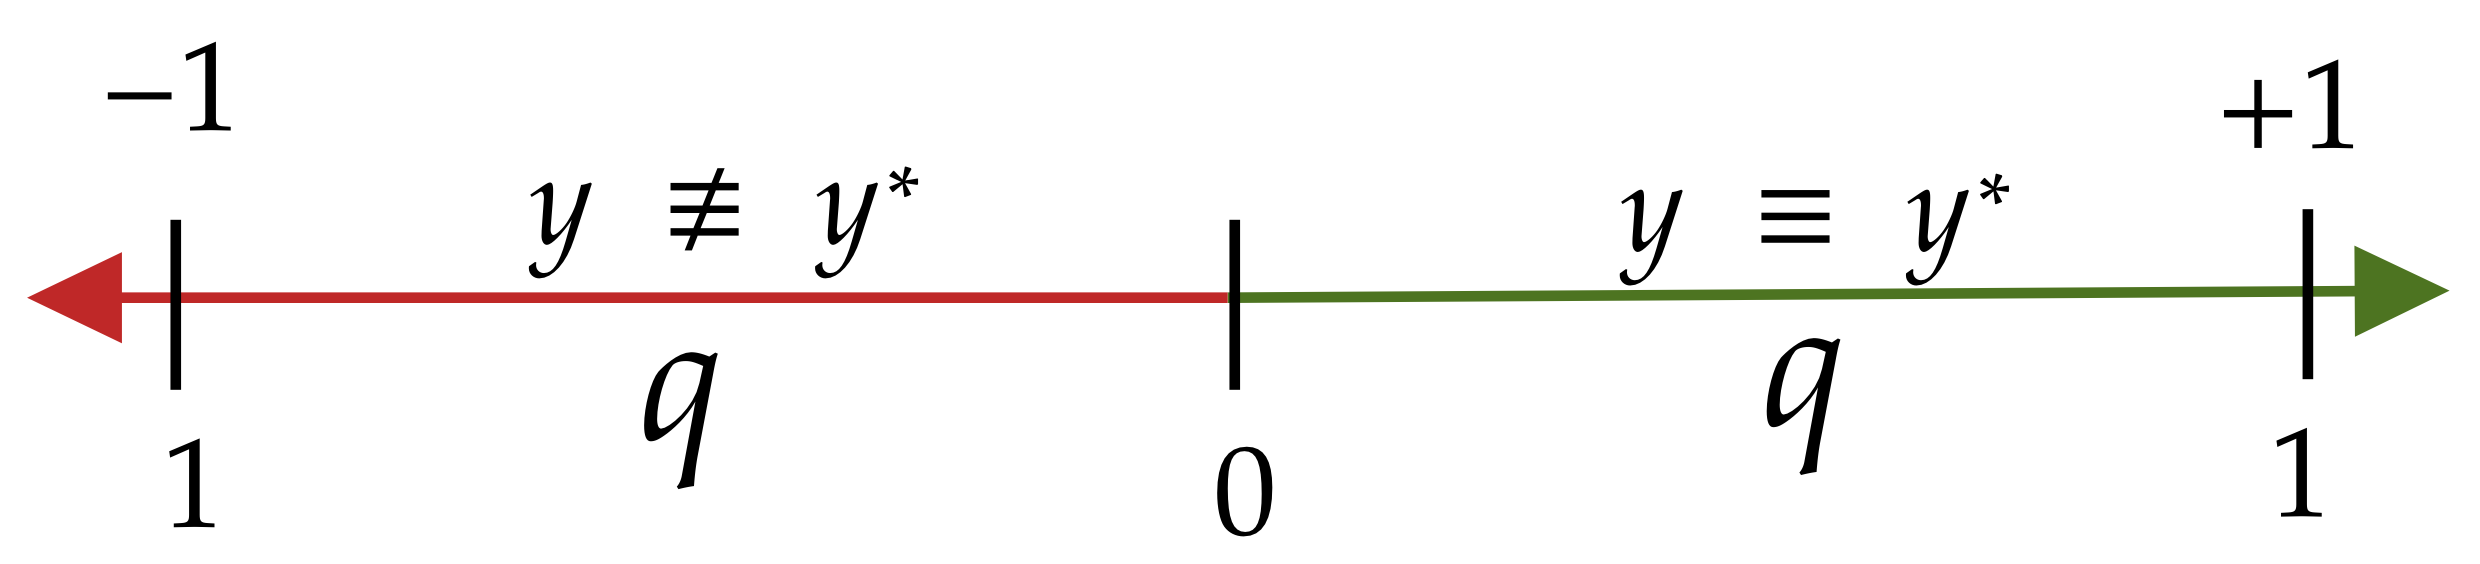
\includegraphics[width=0.9\linewidth]{figures/brier_score_visualization.png}
    \caption{Illustration of the Brier score when adapted to free-form response with answer $y$ and probability $q$.}
    \label{fig:brier_score_visualization}
   
\end{wrapfigure}

which shifts the range from $[-2,0]$ to $[-1,1]$ while providing a more natural interpretation: predicting $q=0$ gives a baseline $0$ regardless of $y$; correct answers receive positive scores, incorrect answers negative scores; and magnitude scales quadratically with confidence. We report $S'$score (visualized in ~\Cref{fig:brier_score_visualization}) as the \emph{Brier score} in this paper. 

Recent work by ~\citet{damani2025beyond} shows that this metric is a proper scoring rule, incentivizing both high accuracy and truthful reporting of probability on the answer that seems most likely. However, note that what we call the Brier score here is distinct from the Brier score considered by \citet{damani2025beyond}. Their Brier score is the one traditionally used for evaluating binary outcomes while ours is for free-form responses. Yet, we can show that our Brier score is \textit{same} as the \textbf{training reward} considered by them.
\clearpage
